\documentclass[accentcolor=tud6b,colorbacktitle,inverttitle,landscape,german,presentation,t]{tudbeamer}
\usepackage[ngerman]{babel}
\usepackage[utf8]{inputenc} 
\usepackage{epstopdf}

\begin{document}

\title[Klassifikation der Schwierigkeitsgrade von Sudokus mit Methoden des maschinellen Lernens]{Klassifikation der Schwierigkeitsgrade von Sudokus mit Methoden des maschinellen Lernens}
\subtitle{Michael Bräunlein\\mbraeunlein@gmail.com}

\author[M. Bräunlein]{Michael Bräunlein}
\institute[Knowledge Engineering TUD]{Knowledge Engineering, TU Darmstadt}

\logo{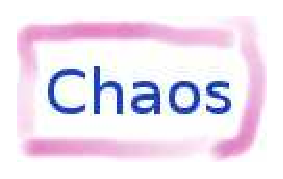
\includegraphics{TUDbeamer-logo}}

\date{17 April 2014}

\begin{titleframe}
\end{titleframe}

\section{Einleitung}
	\begin{frame}
	\frametitle{Einleitung}
	\begin{itemize}
	\item Sudokus finden sich überall
	\item Unterschiedliche Bewertungsskalen
	\item Unterschiedliche Einteilungsverfahren
	\item Bisher kein Verfahren zur Einteilung mit maschinellem Lernen
	\item Sudokus sind zur Bearbeitung mit Computern prädestiniert
	\end{itemize}
	\end{frame}

\section{Grundlagen}
	\subsection{Regeln}
		\begin{frame}
		\frametitle{Die Regeln}
		\begin{itemize}
		\item Sudoku hat nur eine Regel
		\item In jeder Zeile, jeder Spalte und jedem Block muss jede Ziffer von 1 bis 9 genau einmal vorkommen
		\item Jedes Sudoku hat eine eindeutige Lösung
		\item Das Sudoku gilt dann als gelöst, wenn alle Felder ausgefüllt sind
		\end{itemize}
		\end{frame}

	\subsection{Regeln}
		\begin{frame}
		\frametitle{Die Begriffe}
		\begin{figure}[Hh]
    		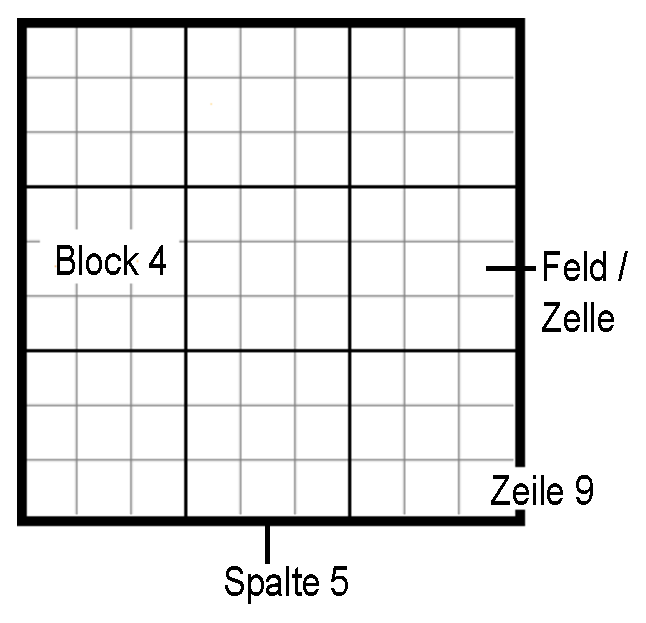
\includegraphics[width=\textwidth,height=\textheight,keepaspectratio]{./img/begriffe.eps}
		\end{figure}
		\end{frame}

	\subsection{Lösungsmethoden}
		\begin{frame}
		\frametitle{Lösungmethoden}
		\begin{itemize}
		\item Jeder Spieler benutzt Lösungsmethoden
		\item Lösungsmethoden sagen viel über den Schwierigkeitsgrad aus
		\item Kandidatenlisten erleichtern das Finden von Zahlenkonstellationen, die Voraussetzung für bestimmte Lösungsmethoden sind
		\item Es gibt viele verschiedene Lösungsmethoden, grob werden zwei Kategorien unterschieden
		\end{itemize}
		\end{frame}

		\subsubsection{Full House}
			\begin{frame}
			\frametitle{Full House}
			\begin{figure}[Hh]
    			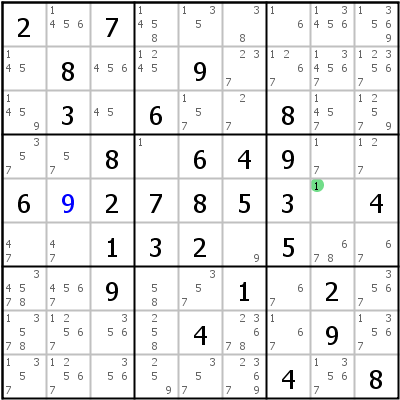
\includegraphics[width=\textwidth,height=\textheight-10pt,keepaspectratio]{./img/full_house.png}
			\end{figure}
			\end{frame}

		\subsubsection{Pointing Pair / Triple}
			\begin{frame}
			\frametitle{Pointing Pair / Triple}
			\begin{figure}[Hh]
    			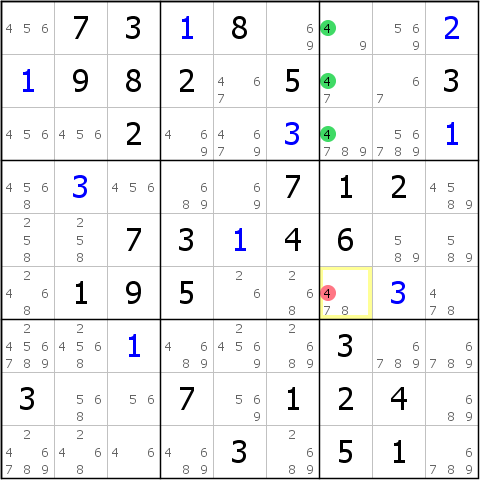
\includegraphics[width=\textwidth,height=\textheight-10pt,keepaspectratio]{./img/pointing_triple.png}
			\end{figure}
			\end{frame}

		\subsubsection{Two-String-Kite}
			\begin{frame}
			\frametitle{Two-String-Kite}
			\begin{figure}[Hh]
    			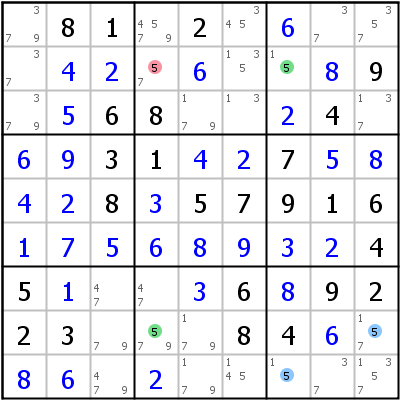
\includegraphics[width=\textwidth,height=\textheight-10pt,keepaspectratio]{./img/2stringkite.png}
			\end{figure}
			\end{frame}

		\subsubsection{XY-Wing}
			\begin{frame}
			\frametitle{XY-Wing}
			\begin{figure}[Hh]
    			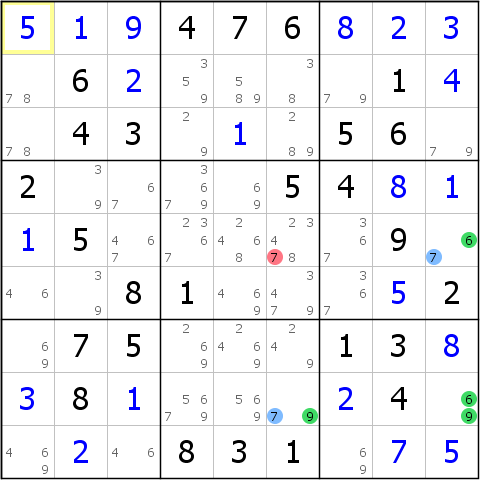
\includegraphics[width=\textwidth,height=\textheight-10pt,keepaspectratio]{./img/XY_Wing.png}
			\end{figure}
			\end{frame}

\section{Klassifikation}
	\subsection{Was sind Featurevectoren}
		\begin{frame}
		\frametitle{Was sind Featurevectoren}
		\begin{itemize}
		\item Merkmalsvektor
		\item n-dimensionaler Vektor
		\item Repräsentation eines Objekts
		\item Ein Eintrag steht für eine Eigenschaft des beschriebenen Sudokus
		\item Featurevektoren sind die Eingabe des Klassifikationsalgorithmus
		\end{itemize}
		\end{frame}

	\subsection{Wie werden Featurevectoren erzeugt}
		\begin{frame}
		\frametitle{Wie werden Featurevectoren erzeugt}
		\begin{itemize}
		\item Am Anfang bekannte Zahlen
		\item Einträge der Kandidatenlisten
		\item Hinzugefügte Zahlen
		\item Entfernte Zahlen
		\item Unterschiedliche Lösungswege für Sudokus möglich
		\item Einfachster Lösungsweg gesucht
		\end{itemize}
		\end{frame}

%%%%%%%%%%%%%%%%%%% Eine Folie mit Effekt %%%%%%%%%%%%%%%%%%%
	\subsection{Entkopplung von konkreten Zahlen}
		\begin{frame}
		\frametitle{Entkopplung von konkreten Zahlen}
		\begin{itemize}
		\item Fast gleiche Sudokus mit vertauschten Zahlen
		\item Gleicher Schwierigkeitsgrad
		\item Unterschiedliche Featurevectoren bei gleichem Lösungsweg
		\end{itemize}
		\end{frame}
	\subsection{Entkopplung von konkreten Zahlen}
		\begin{frame}
		\frametitle{Entkopplung von konkreten Zahlen}
		\begin{itemize}
		\item Fast gleiche Sudokus mit vertauschten Zahlen
		\item Gleicher Schwierigkeitsgrad
		\item Unterschiedliche Featurevectoren bei gleichem Lösungsweg
		\item Lösung?
		\end{itemize}
		\end{frame}
	\subsection{Entkopplung von konkreten Zahlen}
		\begin{frame}
		\frametitle{Entkopplung von konkreten Zahlen}
		\begin{itemize}
		\item Fast gleiche Sudokus mit vertauschten Zahlen
		\item Gleicher Schwierigkeitsgrad
		\item Unterschiedliche Featurevectoren bei gleichem Lösungsweg
		\item Sortierung der Features nach Häufigkeit
		\item Kein relevanter Informationsverlust
		\item Gleicher Featurevector auch bei vertauschten Ziffern
		\end{itemize}
		\end{frame}
%%%%%%%%%%%%%%%%%%%%%%%%%%%%%%%%%%%%%%%%%%%%%%

	\subsection{Entkopplung von konkreten Zahlen (Beispiel)}
		\begin{frame}
		\frametitle{Entkopplung von konkreten Zahlen (Beispiel)}
		\begin{itemize}
		\item Beispiel des Featurevectors einer Methode\\$\mathbf{(1, 0, 4, 15, 3, 0, 9, 2, 0)^{T}}$
		\item Vertauchte Ziffern 7 und 8\\$\mathbf{(1, 0, 4, 15, 3, 0, 2, 9, 0)^{T}}$
		\item Nach der Sortierung nach der Häufigkeit\\$\mathbf{(15, 9, 4, 3, 2, 1, 0, 0, 0)^{T}}$
		\end{itemize}
		\end{frame}

\section{Aufbau}
	\subsection{Software}
		\begin{frame}
		\frametitle{Software}
		\begin{itemize}
		\item Fremdsoftware für Klassifizierer und Lösungsmethoden
		\item Für den Klassifizierer: Weka\footnote{\url{http://www.cs.waikato.ac.nz/ml/weka/}}
		\item Für die Lösungsmethoden: Hodoku\footnote{\url{http://hodoku.sourceforge.net/de/index.php}}
		\item Beide Projekte stehen unter der GPLv3 Lizenz
		\item Eigene Software in Java
		\item Extrahierung der Featurevectoren und Verbindung der Projekte
		\end{itemize}
		\end{frame}

\section{Ergebnisse}


\end{document}

